\newcommand{\erdatamodaler}{ERwin Data Modeler~}

\chapter{РАЗРАБОТКА ФУНКЦИОНАЛЬНОЙ И \\СТРУКТУРНОЙ СХЕМ УЗЛА}

К разработке предлагается устройство ресинхронизации данных. Определим структурные элементы устройства, принцип и порядок его работы.

\section{Описание принципа работы}
Взаимодействие с устройством производится посредством передачи восьмибитного слова на вход wdata. Аппаратный блок осуществляет запись данных во внутреннюю память по сигналам тактового генератора домена источника данных wclk, основываясь на состоянии входных сигналов wrst, wen и служебных сигналов wr\_full,  wptr, rptr.

Устройство может одновременно хранить шестнадцать восьмибитных слов, используя для их адресации пятиразрядный адрес, в котором старший бит призван реализовать возможность контроля заполнения и опустошения очереди.

Чтение из устройства ресинхронизации производится посредством считывания тридцатидвухразрядного слова, генерируемого на выходе rdata. Аппаратный блок осуществляет чтение данных из внутренней памяти по сигналам тактового генератора домена получателя данных, основываясь на состоянии входных сигналов rrst, ren  r\_empty wptr, rptr, rdredy.

Тактовые сигналы входного и выходного каналов независимы, однако тактовая частота для выхода очереди составляет как минимум   $\dfrac14$ от тактовой частоты входного интерфейса FIFO.

Устройство 


\section{функциональная схема узла}
Предлагается для построения устройства ресинхронизации данных, работающего в режиме очереди с независимыми тактовыми сигналами, использовать данную функциональную схему (см. Рисунок \ref{fig:unit-design}).

\begin{figure}
	\centering
	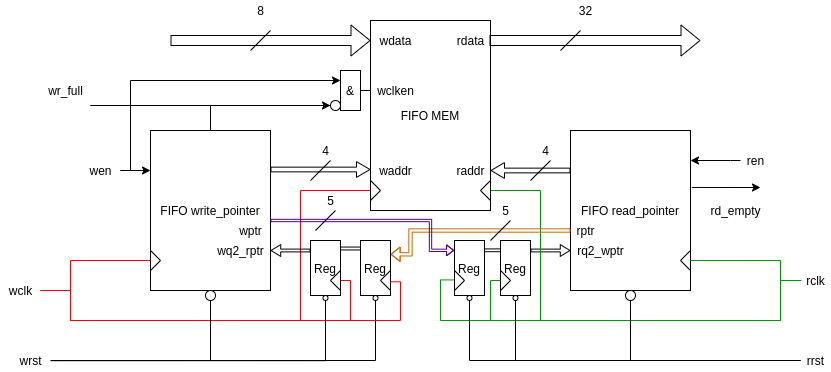
\includegraphics[width=1\linewidth]{course-scheme/images/unit-design}
	\caption{Функциональная схема устройства}
	\label{fig:unit-design}
\end{figure}


Приведем описание входов, выходов и служебных сигналов устройства.


\begin{table}[htbp]
	\caption{}
	\centering
	\fontsize{12}{16pt}\selectfont
	\begin{tabular}{|l|l|}
		\hline
		\multicolumn{1}{|c}{\textbf{Название}} & \multicolumn{1}{|c|}{\textbf{Назначение}} \\ \hline
		asize  &  размер адреса данных с учетом адресации MSB \\ \hline
		dsize  &  размер данных в битах \\ \hline
		mem  &  ячейки памяти очереди \\ \hline
		rbin  &  текущий адрес чтения в бинарном коде \\ \hline
		rbinnext  &  адрес чтения в бинарном коде в следующем такте \\ \hline
		rclk  &  тактирование на чтение данных \\ \hline
		rdata  &  данные на чтение \\ \hline
		rden  &  разрешение на чтение \\ \hline
		rdredy  &  готовность выдать данные \\ \hline
		rempty  &  сигнал пустоты очереди (прочтено все, что записано) \\ \hline
		rempty\_next  &  пустота очереди на следующем такте \\ \hline
		rgray  &  текущий адрес чтения в коде Грея \\ \hline
		rgraynext  &  адрес чтения в коде Грея в следующем такте \\ \hline
		rq1\_wgray  &  адрес чтения в первом синхро-триггере \\ \hline
		rq2\_wgray  &  адрес чтения во втором синхро-триггере \\ \hline
		rrstn  &  сброс указателя чтения \\ \hline
		wbin  &  текущий адрес записи в бинарном коде \\ \hline
		wbinnext  &  адрес записи в бинарном коде в следующем такте \\ \hline
		wclk  &  Тактирование на запись данных \\ \hline
		wdata  &  данные на запись \\ \hline
		wfull  &  сигнал заполнения очереди \\ \hline
		wfull\_next  &  заполненность очереди на следующем такте \\ \hline
		wgray  &  текущий адрес записи в коде Грея \\ \hline
		wgraynext  &  адрес записи в коде Грея в следующем такте \\ \hline
		wq1\_rgray  &  адрес записи в первом синхро-триггере \\ \hline
		wq2\_rgray  &  адрес записи во втором синхро-триггере \\ \hline
		wren  &  разрешение на запись \\ \hline
		wrstn  &  сброc указателя записи \\ \hline
	\end{tabular}
	\label{}
\end{table}





\clearpage